\documentclass{beamer}

\usepackage{amsmath}

\usetheme{AnnArbor}
\usecolortheme{crane}
\usefonttheme[onlymath]{serif}

\title{Deep Learning - Foundations and Concepts}
\subtitle{Chapter 19. Autoencoders}
\author{nonlineark@github}
\date{\today}

\begin{document}

\begin{frame}
    \titlepage
\end{frame}

\begin{frame}
    \frametitle{Outline}
    \tableofcontents
\end{frame}

\section{Deterministic Autoencoders}

\begin{frame}
    \frametitle{Linear autoencoders}
    \begin{figure}
        \caption{An autoencoder neural network having two layers of weights}
        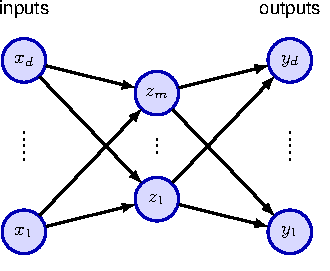
\includegraphics{Figure_1.pdf}
    \end{figure}
\end{frame}

\begin{frame}
    \frametitle{Linear autoencoders}
    Consider a two-layer neural network having $D$ inputs, $D$ output units and $M$ hidden units, with $M<D$. The targets used to train the network are simply the input vectors themselves, so that the network attempts to map each input vector onto itself. We choose a sum-of-squares error of the form:
    \begin{equation*}
        E(w)=\frac{1}{2}\sum_{n=1}^{N}||y(x_{n};w)-x_{n}||^{2}
    \end{equation*}
\end{frame}

\begin{frame}
    \frametitle{Linear autoencoders}
    \begin{itemize}
        \item If the hidden units have linear activation functions, then it can be shown that when the error function is minimized, the network performs a projection onto the $M$-dimensional subspace that is spanned by the first $M$ principal components of the data.
        \item Even with nonlinear hidden units, the minimum error solution is again given by the projection onto the principal component subspace. There is therefore no advantage in using two-layer neural networks to perform dimensionality reduction.
    \end{itemize}
\end{frame}

\begin{frame}
    \frametitle{Deep autoencoders}
    \begin{figure}
        \caption{A four-layer auto-associative network that can perform a nonlinear dimensionality reduction}
        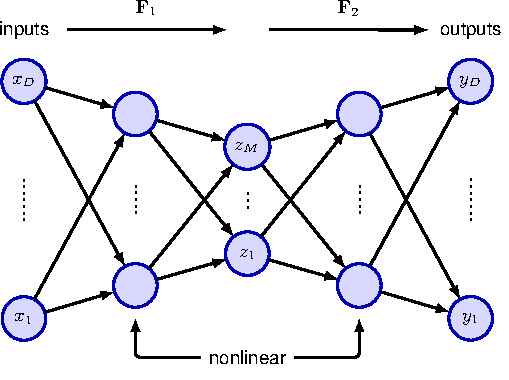
\includegraphics[height=0.6\textheight]{Figure_2.pdf}
    \end{figure}
\end{frame}

\begin{frame}
    \frametitle{Deep autoencoders}
    Consider the four-layer auto-associative network shown on the previous slide:
    \begin{itemize}
        \item The output units are linear, and the $M$ units in the second layer can also be linear.
        \item However, the first and third layers have sigmoidal nonlinear activation functions.
    \end{itemize}
    We can view this network as two successive functional mappings $F_{1}$ and $F_{2}$:
    \begin{itemize}
        \item $F_{1}$ projects the original $D$-dimensional data onto an $M$-dimensional subspace defined by the activations of the units in the second layer.
        \item $F_{2}$ maps from the $M$-dimensional hidden space back into the original $D$-dimensional input space.
    \end{itemize}
\end{frame}

\begin{frame}
    \frametitle{Deep autoencoders}
    \begin{itemize}
        \item Such a network effectively performs a nonlinear form of PCA.
        \item However:
        \begin{itemize}
            \item Training the network now involves a nonlinear optimization, and computationally intensive nonlinear optimization techniques must be used.
            \item There is the risk of finding a sub-optimal local minimum of the error function.
            \item The dimensionality of the subspace must be specified before training the network.
        \end{itemize}
    \end{itemize}
\end{frame}

\begin{frame}
    \frametitle{Sparse autoencoders}
    Instead of limiting the number of nodes in one of the hidden layers in the network, an alternative way to constrain the internal representation is to use a regularizer to encourage a sparse representation:
    \begin{equation*}
        \tilde{E}(w)=E(w)+\lambda\sum_{k=1}^{K}|z_{k}|
    \end{equation*}
    where $E(w)$ is the unregularized error, and the sum over $k$ is taken over the activation values of all the units in one of the hidden layers.
\end{frame}

\begin{frame}
    \frametitle{Denoising autoencoders}
    The idea of denoising autoencoders is to take each input vector $x_{n}$ and to corrupt it with noise to give a modified vector $\tilde{x}_{n}$ which is then input to an autoencoder to give an output $y(\tilde{x}_{n};w)$. The network is trained to reconstruct the original noise-free input vector:
    \begin{equation*}
        E(w)=\sum_{n=1}^{N}||y(\tilde{x}_{n};w)-x_{n}||^{2}
    \end{equation*}
\end{frame}

\begin{frame}
    \frametitle{Denoising autoencoders}
    \begin{itemize}
        \item One form of noise involves setting a randomly chosen subset of the input variables to zero.
        \item An alternative approach is to add independent zero-mean Gaussian noise to every input variable, where the scale of the noise is set by the variance of the Gaussian.
    \end{itemize}
\end{frame}

\begin{frame}
    \frametitle{Masked autoencoders}
    \begin{itemize}
        \item In a masked autoencoder, a deep network is used to reconstruct an image given a corrupted version of that image as input. The form of corruption is masking, or dropping out, part of the input image.
        \item This technique is generally used in combination with a vision transformer architecture.
        \item Compared to language, images have much more redundancy along with strong local correlations. The best internal representations are learned when a relatively high proportion of the input image is masked, typically $75\%$.
        \item The decoder is discarded and the encoder is applied to the full image with no masking and with a fresh set of output layers that are fine-tuned for the required application.
    \end{itemize}
\end{frame}

\begin{frame}
    \frametitle{Masked autoencoders}
    \begin{figure}
        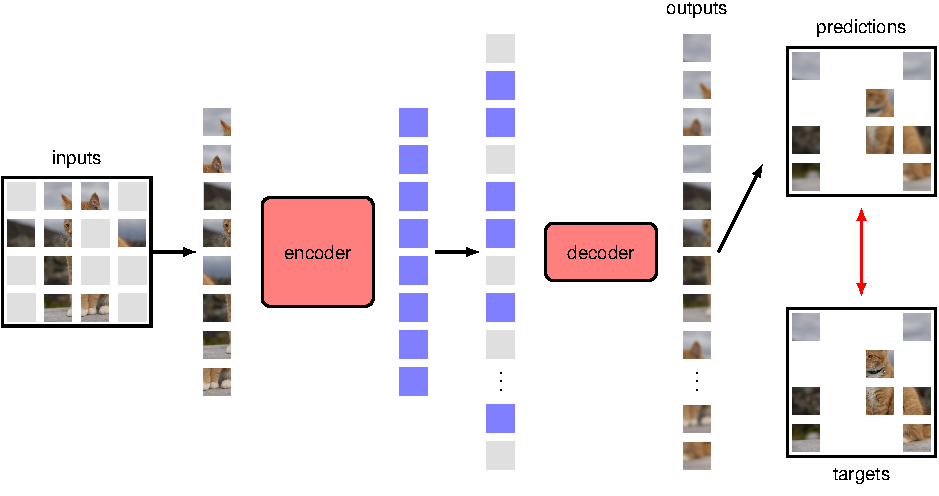
\includegraphics[width=0.8\textwidth]{Figure_5.pdf}
    \end{figure}
\end{frame}

\end{document}